% Source: Code/ML_overlay/ir_rgb_registration/paper/figures/fig_affine_head_detail.tex
% AffineHead Detail: GAP + MLP with Identity Initialization
% IR/RGB Registration — Journal Figure
\documentclass[tikz,border=4pt]{standalone}

\usepackage[T1]{fontenc}
\usepackage{lmodern}
\usepackage{amsmath}

\usetikzlibrary{arrows.meta, positioning, calc, fit, decorations.pathreplacing, shapes.geometric}

% --- Brand Colors ---
\definecolor{Garnet}{HTML}{73000A}
\definecolor{Atlantic}{HTML}{466A9F}
\definecolor{Congaree}{HTML}{1F414D}
\definecolor{Rose}{HTML}{CC2E40}
\definecolor{Honeycomb}{HTML}{A49137}
\definecolor{WarmGrey}{HTML}{676156}
\definecolor{Black90}{HTML}{363636}
\definecolor{Black70}{HTML}{5C5C5C}
\definecolor{Black50}{HTML}{A2A2A2}
\definecolor{Black30}{HTML}{C7C7C7}
\definecolor{Black10}{HTML}{ECECEC}
\definecolor{Horseshoe}{HTML}{65780B}

\begin{document}
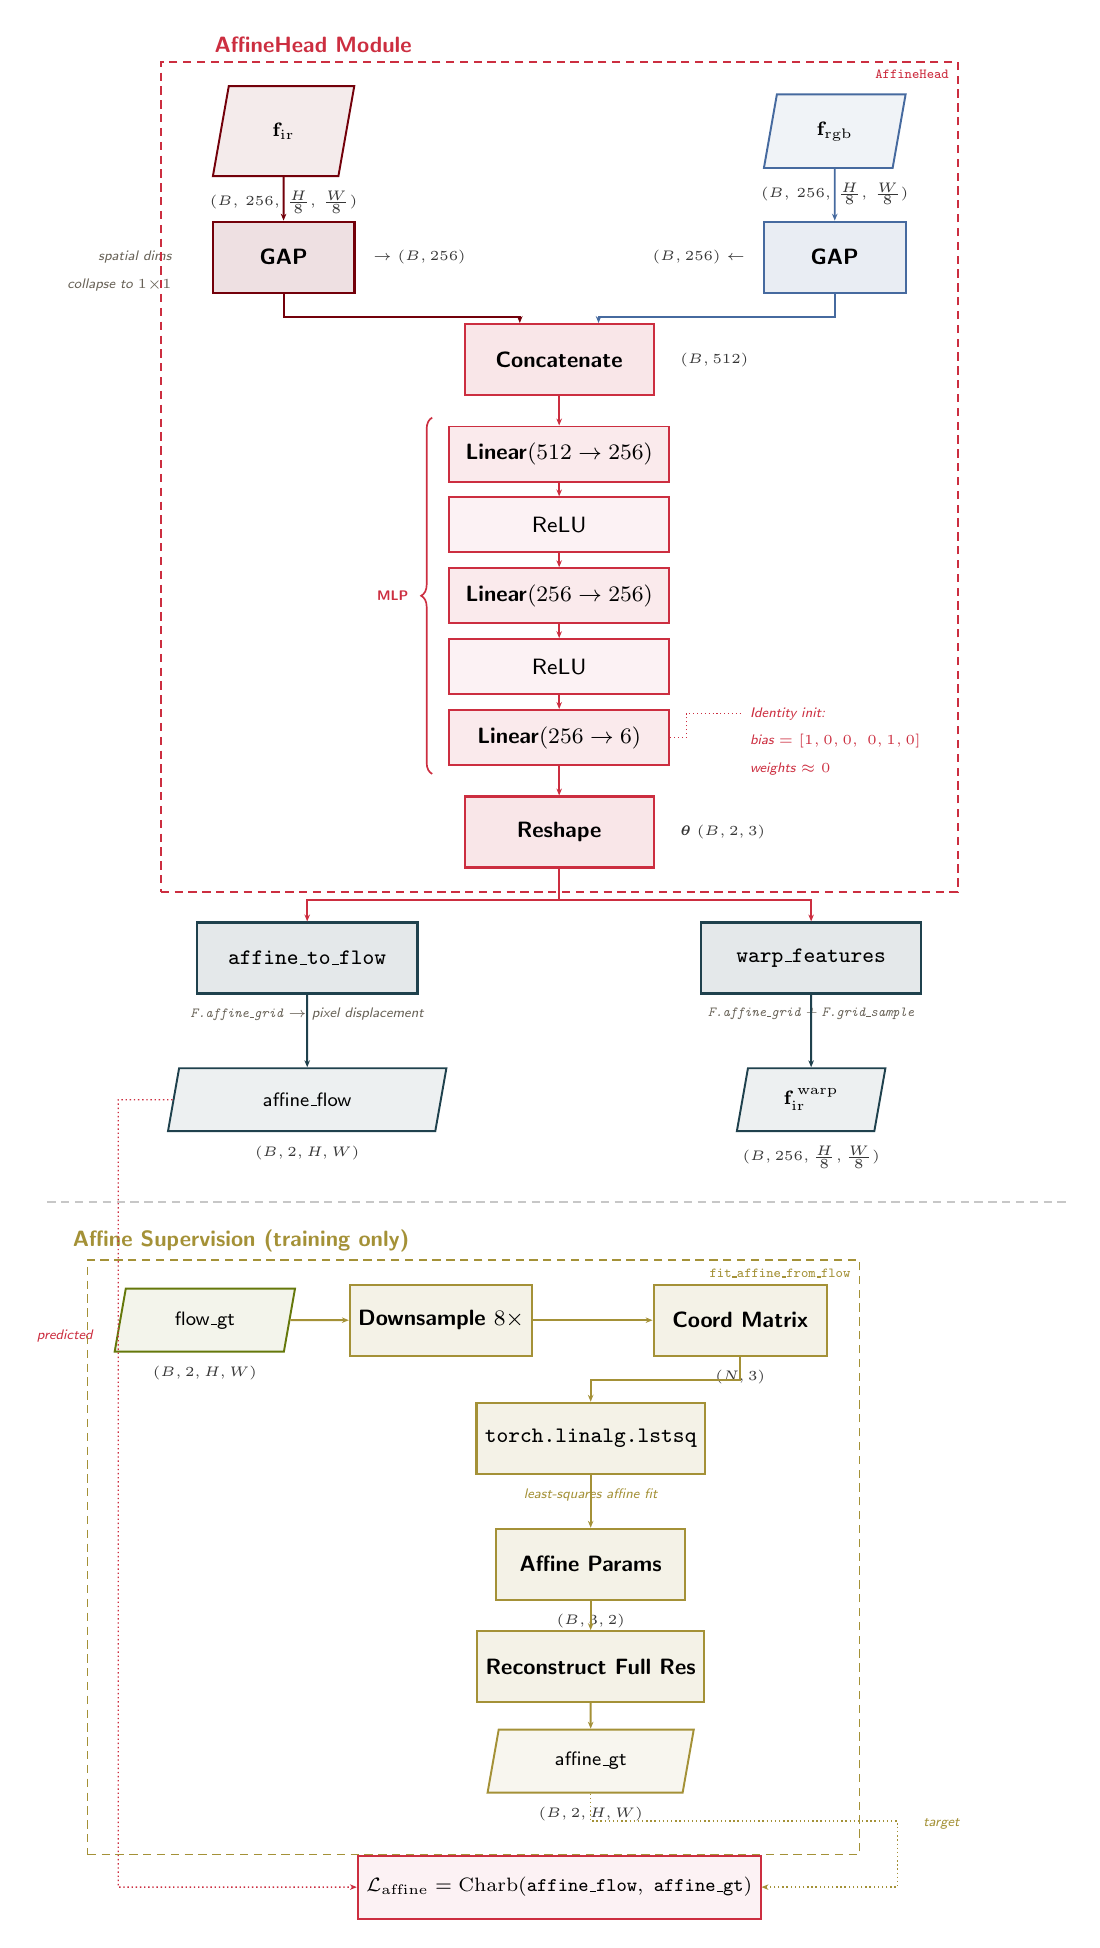
\begin{tikzpicture}[
    >=Stealth,
    font=\sffamily\small,
    % --- Processing block ---
    procblock/.style={
        draw=#1, fill=#1!12, line width=0.8pt,
        minimum height=9mm, minimum width=22mm,
        inner sep=3pt, align=center,
        font=\sffamily\footnotesize\bfseries,
    },
    % --- MLP layer block (narrower) ---
    mlpblock/.style={
        draw=Rose, fill=Rose!10, line width=0.7pt,
        minimum height=7mm, minimum width=28mm,
        inner sep=2pt, align=center,
        font=\sffamily\footnotesize,
    },
    % --- Data tensor ---
    tensor/.style={
        draw=#1, fill=#1!8, line width=0.7pt,
        minimum height=8mm, minimum width=18mm,
        inner sep=2pt, align=center,
        font=\sffamily\scriptsize,
        shape=trapezium,
        trapezium left angle=80, trapezium right angle=100,
    },
    % --- Dimension annotation ---
    dimlab/.style={
        font=\sffamily\tiny, text=Black90,
    },
    % --- Arrow styles ---
    dataarrow/.style={
        -{Stealth[length=2.5pt,width=2pt]},
        line width=0.7pt, color=#1,
    },
    % --- Annotation callout ---
    annot/.style={
        font=\sffamily\tiny\itshape, text=WarmGrey,
        align=left,
    },
    % --- Section title ---
    sectitle/.style={
        font=\sffamily\footnotesize\bfseries, text=#1,
    },
]

% =====================================================================
% SECTION TITLE
% =====================================================================
\node[sectitle=Rose, anchor=west] (title) at (-4.5, 0.4) {\textsf{AffineHead Module}};

% =====================================================================
% ROW 0: INPUT FEATURE MAPS
% =====================================================================
% IR feature map
\node[tensor=Garnet] (fmap_ir) at (-3.5, -0.7) {$\mathbf{f}_{\mathrm{ir}}$};
\node[dimlab, below=0.5mm of fmap_ir] (dim_fir) {$(B,\,256,\,\frac{H}{8},\,\frac{W}{8})$};

% RGB feature map
\node[tensor=Atlantic] (fmap_rgb) at (3.5, -0.7) {$\mathbf{f}_{\mathrm{rgb}}$};
\node[dimlab, below=0.5mm of fmap_rgb] (dim_frgb) {$(B,\,256,\,\frac{H}{8},\,\frac{W}{8})$};

% =====================================================================
% ROW 1: GLOBAL AVERAGE POOLING
% =====================================================================
\node[procblock=Garnet, minimum width=18mm] (gap_ir) at (-3.5, -2.3) {GAP};
\node[dimlab, right=1mm of gap_ir, anchor=west] {$\to (B, 256)$};

\node[procblock=Atlantic, minimum width=18mm] (gap_rgb) at (3.5, -2.3) {GAP};
\node[dimlab, left=1mm of gap_rgb, anchor=east] {$(B, 256) \leftarrow$};

% GAP description
\node[annot, anchor=east] at (-4.8, -2.3) {spatial dims};
\node[annot, anchor=east] at (-4.8, -2.65) {collapse to $1{\times}1$};

% Arrows: fmaps to GAP
\draw[dataarrow=Garnet] (fmap_ir.south) -- (gap_ir.north);
\draw[dataarrow=Atlantic] (fmap_rgb.south) -- (gap_rgb.north);

% =====================================================================
% ROW 2: CONCATENATION
% =====================================================================
\node[procblock=Rose, minimum width=24mm] (concat) at (0, -3.6) {Concatenate};
\node[dimlab, right=2mm of concat, anchor=west] {$(B, 512)$};

% Arrows: GAP to concat
\draw[dataarrow=Garnet] (gap_ir.south) -- ++(0,-3mm) -| ($(concat.north) + (-5mm,0)$);
\draw[dataarrow=Atlantic] (gap_rgb.south) -- ++(0,-3mm) -| ($(concat.north) + (5mm,0)$);

% =====================================================================
% ROWS 3--7: MLP LAYERS
% =====================================================================
\node[mlpblock] (fc1) at (0, -4.8) {\textbf{Linear}$(512 \to 256)$};
\node[mlpblock, fill=Rose!6] (relu1) at (0, -5.7) {ReLU};
\node[mlpblock] (fc2) at (0, -6.6) {\textbf{Linear}$(256 \to 256)$};
\node[mlpblock, fill=Rose!6] (relu2) at (0, -7.5) {ReLU};
\node[mlpblock] (fc3) at (0, -8.4) {\textbf{Linear}$(256 \to 6)$};

% Identity initialization annotation
\node[annot, anchor=west, text=Rose] (init_note) at (2.3, -8.1)
    {Identity init:};
\node[annot, anchor=west, text=Rose] at (2.3, -8.45)
    {bias $= [1,0,0,\;0,1,0]$};
\node[annot, anchor=west, text=Rose] at (2.3, -8.8)
    {weights $\approx 0$};
\draw[Rose, line width=0.4pt, densely dotted]
    (fc3.east) -- ++(2mm,0) |- (init_note.west);

% MLP brace
\draw[decorate, decoration={brace, amplitude=4pt, mirror},
      line width=0.6pt, draw=Rose]
    ($(fc1.north west) + (-2mm, 1mm)$) -- ($(fc3.south west) + (-2mm, -1mm)$)
    node[midway, left=5pt, sectitle=Rose, align=center, font=\sffamily\tiny\bfseries] {MLP};

% Arrows within MLP
\draw[dataarrow=Rose] (concat.south) -- (fc1.north);
\draw[dataarrow=Rose] (fc1.south) -- (relu1.north);
\draw[dataarrow=Rose] (relu1.south) -- (fc2.north);
\draw[dataarrow=Rose] (fc2.south) -- (relu2.north);
\draw[dataarrow=Rose] (relu2.south) -- (fc3.north);

% =====================================================================
% ROW 8: RESHAPE TO THETA
% =====================================================================
\node[procblock=Rose, minimum width=24mm] (reshape) at (0, -9.6) {Reshape};
\node[dimlab, right=2mm of reshape, anchor=west] {$\boldsymbol{\theta}\;(B, 2, 3)$};

\draw[dataarrow=Rose] (fc3.south) -- (reshape.south |- fc3.south) -- (reshape.north);

% =====================================================================
% ROW 9: TWO OUTPUT BRANCHES
% =====================================================================
% Left branch: affine_to_flow
\node[procblock=Congaree, minimum width=28mm] (aff2flow) at (-3.2, -11.2)
    {\texttt{affine\_to\_flow}};
\node[annot, below=0.5mm of aff2flow] {%
    \texttt{F.affine\_grid} $\to$ pixel displacement};

% Right branch: warp_features
\node[procblock=Congaree, minimum width=28mm] (warpfeat) at (3.2, -11.2)
    {\texttt{warp\_features}};
\node[annot, below=0.5mm of warpfeat] {%
    \texttt{F.affine\_grid} + \texttt{F.grid\_sample}};

% Arrows: theta to branches
\draw[dataarrow=Rose] (reshape.south) -- ++(0,-4mm) -| (aff2flow.north);
\draw[dataarrow=Rose] (reshape.south) -- ++(0,-4mm) -| (warpfeat.north);

% Branch outputs
\node[tensor=Congaree] (flow_aff) at (-3.2, -13.0) {affine\_flow};
\node[dimlab, below=0.5mm of flow_aff] {$(B, 2, H, W)$};

\node[tensor=Congaree] (fmap_warp) at (3.2, -13.0) {$\mathbf{f}_{\mathrm{ir}}^{\,\mathrm{warp}}$};
\node[dimlab, below=0.5mm of fmap_warp] {$(B, 256, \frac{H}{8}, \frac{W}{8})$};

\draw[dataarrow=Congaree] (aff2flow.south) -- (flow_aff.north);
\draw[dataarrow=Congaree] (warpfeat.south) -- (fmap_warp.north);

% =====================================================================
% DASHED BOUNDING BOX: AffineHead module
% =====================================================================
\node[draw=Rose, densely dashed, line width=0.7pt,
      inner xsep=5mm, inner ysep=3mm,
      fit=(fmap_ir)(fmap_rgb)(gap_ir)(gap_rgb)(concat)(fc3)(reshape)(dim_fir)(dim_frgb),
      label={[sectitle=Rose, anchor=north east, font=\sffamily\tiny\bfseries]north east:{\texttt{AffineHead}}}] {};

% =====================================================================
% SEPARATOR LINE
% =====================================================================
\draw[Black30, line width=0.5pt, densely dashed]
    (-6.5, -14.3) -- (6.5, -14.3);
\node[sectitle=Honeycomb, anchor=west] at (-6.3, -14.8)
    {Affine Supervision (training only)};

% =====================================================================
% SUB-DIAGRAM: fit_affine_from_flow (lstsq fitting)
% =====================================================================
% Input: GT flow
\node[tensor=Horseshoe] (flow_gt) at (-4.5, -15.8) {flow\_gt};
\node[dimlab, below=0.5mm of flow_gt] {$(B, 2, H, W)$};

% Step 1: downsample
\node[procblock=Honeycomb, minimum width=22mm] (ds8) at (-1.5, -15.8)
    {Downsample $8\times$};
\draw[dataarrow=Honeycomb] (flow_gt.east) -- (ds8.west);

% Step 2: build coord matrix
\node[procblock=Honeycomb, minimum width=22mm] (coords) at (2.3, -15.8)
    {Coord Matrix};
\node[dimlab, below=0.5mm of coords] {$(N, 3)$};
\draw[dataarrow=Honeycomb] (ds8.east) -- (coords.west);

% Step 3: lstsq
\node[procblock=Honeycomb, minimum width=24mm, font=\sffamily\footnotesize\bfseries]
    (lstsq) at (0.4, -17.3) {\texttt{torch.linalg.lstsq}};
\node[annot, text=Honeycomb, below=0.5mm of lstsq]
    {least-squares affine fit};
\draw[dataarrow=Honeycomb] (coords.south) -- ++(0,-3mm) -| (lstsq.north);

% Step 4: affine params
\node[procblock=Honeycomb, minimum width=24mm] (aff_params) at (0.4, -18.9)
    {Affine Params};
\node[dimlab, below=0.5mm of aff_params] {$(B, 3, 2)$};
\draw[dataarrow=Honeycomb] (lstsq.south) -- (aff_params.north);

% Step 5: reconstruct full-res flow
\node[procblock=Honeycomb, minimum width=28mm] (recon) at (0.4, -20.2)
    {Reconstruct Full Res};
\draw[dataarrow=Honeycomb] (aff_params.south) -- (recon.north);

% Output: affine_gt
\node[tensor=Honeycomb] (aff_gt) at (0.4, -21.4) {affine\_gt};
\node[dimlab, below=0.5mm of aff_gt] (dim_affgt) {$(B, 2, H, W)$};
\draw[dataarrow=Honeycomb] (recon.south) -- (aff_gt.north);

% Comparison: loss node centered below the lower section
\node[draw=Rose, fill=Rose!6, line width=0.7pt,
      minimum height=8mm, minimum width=42mm,
      inner sep=3pt, align=center,
      font=\sffamily\scriptsize] (compare) at (0, -23.0)
    {$\mathcal{L}_{\mathrm{affine}} = \mathrm{Charb}(\texttt{affine\_flow},\; \texttt{affine\_gt})$};
% Arrow from affine_flow: exit west, go to margin, then south to loss.west
\draw[Rose, line width=0.5pt, densely dotted, -{Stealth[length=2.5pt,width=2pt]}]
    (flow_aff.west) -- (-5.6,-13.0)
    -- (-5.6,-23.0) -- (compare.west);
\node[annot, text=Rose, anchor=east, font=\sffamily\tiny\itshape]
    at (-5.8,-16.0) {predicted};
% Arrow from affine_gt: down then right margin channel to loss.east
\draw[Honeycomb, line width=0.5pt, densely dotted, -{Stealth[length=2.5pt,width=2pt]}]
    (aff_gt.south) -- ++(0,-3.5mm)
    -| (4.3,-22.2) -- (4.3,-23.0) -- (compare.east);
\node[annot, text=Honeycomb, anchor=west, font=\sffamily\tiny\itshape]
    at (4.5,-22.2) {target};

% =====================================================================
% UTILITY LABEL
% =====================================================================
\node[draw=Honeycomb, densely dashed, line width=0.5pt,
      inner xsep=4mm, inner ysep=3mm,
      fit=(flow_gt)(ds8)(coords)(lstsq)(aff_params)(recon)(aff_gt)(dim_affgt),
      label={[sectitle=Honeycomb, anchor=north east, font=\sffamily\tiny\bfseries]north east:{\texttt{fit\_affine\_from\_flow}}}] {};

\end{tikzpicture}
\end{document}
